\documentclass{ximera}

%\usepackage{todonotes}

\newcommand{\todo}{}

\usepackage{tkz-euclide}
\tikzset{>=stealth} %% cool arrow head
\tikzset{shorten <>/.style={ shorten >=#1, shorten <=#1 } } %% allows shorter vectors

\usepackage{tkz-tab}  %% sign charts
\usetikzlibrary{decorations.pathreplacing} 

\usetikzlibrary{backgrounds} %% for boxes around graphs
\usetikzlibrary{shapes,positioning}  %% Clouds and stars
\usetikzlibrary{matrix} %% for matrix
\usepgfplotslibrary{polar} %% for polar plots
\usetkzobj{all}
\usepackage[makeroom]{cancel} %% for strike outs
%\usepackage{mathtools} %% for pretty underbrace % Breaks Ximera
\usepackage{multicol}

\usepackage{polynom}



\usepackage[many]{tcolorbox}  %% for titled boxes
\newtcolorbox{xbox}[1]{%
    tikznode boxed title,
    enhanced,
    arc=0mm,
    interior style={white},
    attach boxed title to top center= {yshift=-\tcboxedtitleheight/2},
    fonttitle=\bfseries,
    colbacktitle=white,coltitle=black,
    boxed title style={size=normal,colframe=white,boxrule=0pt},
    title={#1}}


\usepackage{array}
\setlength{\extrarowheight}{+.1cm}   
\newdimen\digitwidth
\settowidth\digitwidth{9}
\def\divrule#1#2{
\noalign{\moveright#1\digitwidth
\vbox{\hrule width#2\digitwidth}}}





\newcommand{\RR}{\mathbb R}
\newcommand{\R}{\mathbb R}
\newcommand{\N}{\mathbb N}
\newcommand{\Z}{\mathbb Z}

%\renewcommand{\d}{\,d\!}
\renewcommand{\d}{\mathop{}\!d}
\newcommand{\dd}[2][]{\frac{\d #1}{\d #2}}
\newcommand{\pp}[2][]{\frac{\partial #1}{\partial #2}}
\renewcommand{\l}{\ell}
\newcommand{\ddx}{\frac{d}{\d x}}
\newcommand{\ddt}{\frac{d}{\d t}}

\newcommand{\zeroOverZero}{\ensuremath{\boldsymbol{\tfrac{0}{0}}}}
\newcommand{\inftyOverInfty}{\ensuremath{\boldsymbol{\tfrac{\infty}{\infty}}}}
\newcommand{\zeroOverInfty}{\ensuremath{\boldsymbol{\tfrac{0}{\infty}}}}
\newcommand{\zeroTimesInfty}{\ensuremath{\small\boldsymbol{0\cdot \infty}}}
\newcommand{\inftyMinusInfty}{\ensuremath{\small\boldsymbol{\infty - \infty}}}
\newcommand{\oneToInfty}{\ensuremath{\boldsymbol{1^\infty}}}
\newcommand{\zeroToZero}{\ensuremath{\boldsymbol{0^0}}}
\newcommand{\inftyToZero}{\ensuremath{\boldsymbol{\infty^0}}}



\newcommand{\numOverZero}{\ensuremath{\boldsymbol{\tfrac{\#}{0}}}}
\newcommand{\dfn}{\textbf}
%\newcommand{\unit}{\,\mathrm}
\newcommand{\unit}{\mathop{}\!\mathrm}
\newcommand{\eval}[1]{\bigg[ #1 \bigg]}
\newcommand{\seq}[1]{\left( #1 \right)}
\renewcommand{\epsilon}{\varepsilon}
\renewcommand{\iff}{\Leftrightarrow}

\DeclareMathOperator{\arccot}{arccot}
\DeclareMathOperator{\arcsec}{arcsec}
\DeclareMathOperator{\arccsc}{arccsc}
\DeclareMathOperator{\si}{Si}
\DeclareMathOperator{\proj}{proj}
\DeclareMathOperator{\scal}{scal}


\newcommand{\tightoverset}[2]{% for arrow vec
  \mathop{#2}\limits^{\vbox to -.5ex{\kern-0.75ex\hbox{$#1$}\vss}}}
\newcommand{\arrowvec}[1]{\tightoverset{\scriptstyle\rightharpoonup}{#1}}
\renewcommand{\vec}{\mathbf}
\newcommand{\veci}{\vec{i}}
\newcommand{\vecj}{\vec{j}}
\newcommand{\veck}{\vec{k}}
\newcommand{\vecl}{\boldsymbol{\l}}

\newcommand{\dotp}{\bullet}
\newcommand{\cross}{\boldsymbol\times}
\newcommand{\grad}{\boldsymbol\nabla}
\newcommand{\divergence}{\grad\dotp}
\newcommand{\curl}{\grad\cross}
%\DeclareMathOperator{\divergence}{divergence}
%\DeclareMathOperator{\curl}[1]{\grad\cross #1}


\colorlet{textColor}{black} 
\colorlet{background}{white}
\colorlet{penColor}{blue!50!black} % Color of a curve in a plot
\colorlet{penColor2}{red!50!black}% Color of a curve in a plot
\colorlet{penColor3}{red!50!blue} % Color of a curve in a plot
\colorlet{penColor4}{green!50!black} % Color of a curve in a plot
\colorlet{penColor5}{orange!80!black} % Color of a curve in a plot
\colorlet{fill1}{penColor!20} % Color of fill in a plot
\colorlet{fill2}{penColor2!20} % Color of fill in a plot
\colorlet{fillp}{fill1} % Color of positive area
\colorlet{filln}{penColor2!20} % Color of negative area
\colorlet{fill3}{penColor3!20} % Fill
\colorlet{fill4}{penColor4!20} % Fill
\colorlet{fill5}{penColor5!20} % Fill
\colorlet{gridColor}{gray!50} % Color of grid in a plot

\newcommand{\surfaceColor}{violet}
\newcommand{\surfaceColorTwo}{redyellow}
\newcommand{\sliceColor}{greenyellow}




\pgfmathdeclarefunction{gauss}{2}{% gives gaussian
  \pgfmathparse{1/(#2*sqrt(2*pi))*exp(-((x-#1)^2)/(2*#2^2))}%
}


%%%%%%%%%%%%%
%% Vectors
%%%%%%%%%%%%%

%% Simple horiz vectors
\renewcommand{\vector}[1]{\left\langle #1\right\rangle}


%% %% Complex Horiz Vectors with angle brackets
%% \makeatletter
%% \renewcommand{\vector}[2][ , ]{\left\langle%
%%   \def\nextitem{\def\nextitem{#1}}%
%%   \@for \el:=#2\do{\nextitem\el}\right\rangle%
%% }
%% \makeatother

%% %% Vertical Vectors
%% \def\vector#1{\begin{bmatrix}\vecListA#1,,\end{bmatrix}}
%% \def\vecListA#1,{\if,#1,\else #1\cr \expandafter \vecListA \fi}

%%%%%%%%%%%%%
%% End of vectors
%%%%%%%%%%%%%

%\newcommand{\fullwidth}{}
%\newcommand{\normalwidth}{}



%% makes a snazzy t-chart for evaluating functions
%\newenvironment{tchart}{\rowcolors{2}{}{background!90!textColor}\array}{\endarray}

%%This is to help with formatting on future title pages.
\newenvironment{sectionOutcomes}{}{} 



%% Flowchart stuff
%\tikzstyle{startstop} = [rectangle, rounded corners, minimum width=3cm, minimum height=1cm,text centered, draw=black]
%\tikzstyle{question} = [rectangle, minimum width=3cm, minimum height=1cm, text centered, draw=black]
%\tikzstyle{decision} = [trapezium, trapezium left angle=70, trapezium right angle=110, minimum width=3cm, minimum height=1cm, text centered, draw=black]
%\tikzstyle{question} = [rectangle, rounded corners, minimum width=3cm, minimum height=1cm,text centered, draw=black]
%\tikzstyle{process} = [rectangle, minimum width=3cm, minimum height=1cm, text centered, draw=black]
%\tikzstyle{decision} = [trapezium, trapezium left angle=70, trapezium right angle=110, minimum width=3cm, minimum height=1cm, text centered, draw=black]


\outcome{Explain the relationship between differentiability and continuity.}
\outcome{Determine whether a piecewise function is differentiable.}
\title[Dig-In:]{Differentiability implies continuity}

\begin{document}
\begin{abstract}
We see that if a function is differentiable at a point, then it must
be continuous at that point.
\end{abstract}
\maketitle

There are connections between continuity and differentiability.

\begin{theorem}[Differentiability Implies Continuity]\index{differentiability implies continuity}
If $f$ is a differentiable function at $x = a$, then $f$ is continuous
at $x=a$.
\begin{explanation}
To explain why this is true, we are going to use the following
definition of the derivative
\[
f'(a) = \lim_{x\to a} \frac{f(x)-f(a)}{x-a}.
\]

  Assuming that $f'(a)$ exists, we want to show that $f(x)$ is
continuous at $x=a$, hence we must show that
\[
\lim_{x\to a} f(x) = f(a).
\]
Starting with
\[
\lim_{x\to a} \left(f(x) - f(a)\right)
\]
we multiply and divide by $(x-a)$ to get
\begin{align*}
  &= \lim_{x\to a} \left((x-a)\frac{f(x) - f(a)}{x-a}\right) \\
  &= \left(\lim_{x\to a} (x-a) \right) \left(\lim_{x\to a}\frac{f(x) - f(a)}{x-a}\right) &\text{Limit Law.} \\
  &= \answer[given]{0}\cdot f'(a) = \answer[given]{0}.
\end{align*}
Since 
\[
\lim_{x\to a}\left(f(x) - f(a)\right) = 0 ,
\]
we apply the Difference Law to the left hand side
\[
\lim_{x\to a}f(x) - \lim_{x\to a}f(a) = 0 ,
\]
and use continuity of a constant to obtain that
\[
\lim_{x\to a}f(x) - f(a) = 0 .
\]
Next, we add $f(a)$ on both sides and get that
\[
\lim_{x\to a}f(x) = f(a).
\]
Now we see that $\lim_{x\to a} f(x) = f(a)$, and so $f$ is continuous at
$x=a$.
\end{explanation}
\end{theorem}

This theorem is often written as its contrapositive:
\begin{quote}
If $f(x)$ is not continuous at $x=a$, then $f(x)$ is not
differentiable at $x=a$.
\end{quote}


Thus from the theorem above, we see that all differentiable functions
on $\RR$ are continuous on $\RR$. Nevertheless there are continuous
functions on $\RR$ that are not differentiable on $\RR$.

\begin{question}
  Which of the following functions are continuous but not
  differentiable on $\RR$?
  \begin{multipleChoice}
    \choice{$x^2$}
    \choice{$\lfloor x \rfloor$}
    \choice[correct]{$|x|$}
    \choice{$\frac{x^2}{x}$}
  \end{multipleChoice}
\end{question}

\begin{example}
  Consider
  \[
  f(x) = \begin{cases}
          x^2 &\text{if $x<3$,}\\
          mx+b &\text{if $x\ge 3$.}
         \end{cases}
  \]
  What values of $m$ and $b$ make $f$ differentiable at $x=3$?
  \begin{explanation}
    To start, we know that  $f$ must be continuous at $x=3$, since it has to be
    differentiable there. We will start by making $f$  continuous at
    $x=3$. Write with me:
    \begin{align*}
      \lim_{x\to 3^-} f(x) &= \answer[given]{9}\\
      \lim_{x\to 3^+} f(x) &= \answer[given]{m 3 + b}\\
      f(3) &= \answer[given]{m 3 + b}
    \end{align*}
    So for the function to be continuous, we must have
    \[
    m\cdot 3 + b =9.
    \]
    We also must ensure that the function is differentiable at $x=3$. In other words, we have to ensure that the following limit exists

 \[
 \lim_{x\to 3}\frac{f(x)-f(3)}{x-3}.\\
\]
In order to compute this limit, we have to compute the two one-sided limits
 \[
 \lim_{x\to 3^{+}}\frac{f(x)-f(3)}{x-3}\\
\]
and
\[
 \lim_{x\to 3^{-}}\frac{f(x)-f(3)}{x-3},\\
\]
since  $f(x)$ changes expression at $x=3$.
Write with me
     \begin{align*}
        \lim_{x\to 3^{-}}\frac{f(x)-f(3)}{x-3}&= \lim_{x\to 3}\frac{x^2 -9}{x-3}\\
      &= \lim_{x\to 3^{-}}\frac{\cancel{(x-3)}(x+3)}{\cancel{x-3}}\\
      &= \lim_{x\to 3^{-}}\left(x+3\right)\\
      &=6,
    \end{align*}
    and
   \begin{align*}
        \lim_{x\to 3^{+}}\frac{f(x)-f(3)}{x-3}&= \lim_{x\to 3}\frac{mx+b -(3m+b)}{x-3}\\
          &= \lim_{x\to 3^{+}}\frac{mx-3m}{x-3}\\
      &= \lim_{x\to 3^{+}}\frac{m\cancel{(x-3)}}{\cancel{x-3}}\\
      &= \lim_{x\to 3^{+}}m\\
      &=m.
    \end{align*}
    Hence, we must have
   \[
      m=6.
  \]
    Ah! So now the equation that must be satisfied
    \begin{align*}
      9 &= m\cdot 3 + b,\\
    becomes\hspace{0.3in}  9 &= 6\cdot 3 + b.\\
    \end{align*}
   Therefore, $b=\answer[given]{-9}$. Thus setting $m=\answer[given]{6}$ and
    $b=\answer[given]{-9}$ will give us a function that is differentiable (and hence
    continuous) at $x=3$.
   
  \end{explanation}
\end{example}

Can we tell from its graph whether the function is differentiable or not at a point $a$?

\begin{question}
What does the graph of a function $f$ possibly look like when $f$ is not differentiable at $a$?
\begin{explanation}

Each of the figures A-D depicts a function that is not differentiable at $a=1$. 
 \begin{image}
    \begin{tabular}{cc}
      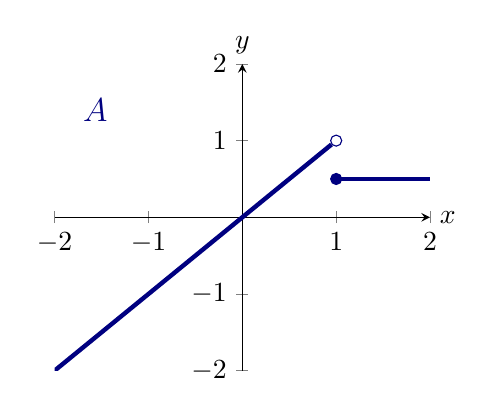
\begin{tikzpicture}
        \begin{axis}[
          domain=-2:2,
          xmin=-2, xmax=2,
          ymin=-2, ymax=2,
          width=2.5in,
          axis lines =middle, xlabel=$x$, ylabel=$y$,
          every axis y label/.style={at=(current axis.above origin),anchor=south},
          every axis x label/.style={at=(current axis.right of origin),anchor=west},
          ]
	  \addplot [ultra thick, penColor, smooth,domain=(-2:0.95)] {x};
	   \addplot [ultra thick, penColor, smooth,domain=(1:2)] {0.5};
	   \addplot[color=penColor,fill=penColor,only marks,mark=*] coordinates{(1,0.5)}; 
	      \addplot[color=penColor,fill=background,only marks,mark=*] coordinates{(1,1)};  %% open hole
          \node at (axis cs:-1.8, 1.4 ) [penColor,anchor=west] {\large$A$};
         
        \end{axis}
      \end{tikzpicture}
      &
      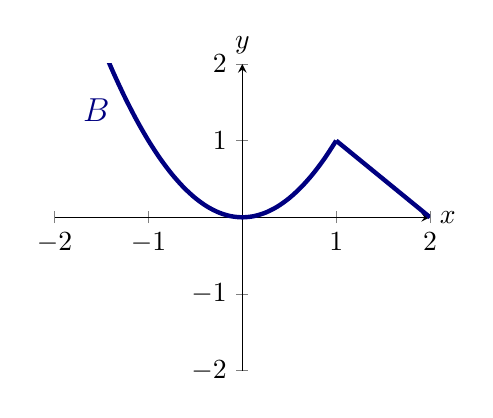
\begin{tikzpicture}
        \begin{axis}[
          domain=-2:2,
          xmin=-2, xmax=2,
          ymin=-2, ymax=2,
          width=2.5in,
          axis lines =middle, xlabel=$x$, ylabel=$y$,
          every axis y label/.style={at=(current axis.above origin),anchor=south},
          every axis x label/.style={at=(current axis.right of origin),anchor=west},
          ]
	  \addplot [ultra thick, penColor, smooth,domain=(1:2)] {2-x};
	    \addplot [ultra thick, penColor, smooth,domain=(-2:1)] {x^2};

          \node at (axis cs:-1.8, 1.4 ) [penColor,anchor=west] {\large$B$};
       
        \end{axis}
      \end{tikzpicture}\\
      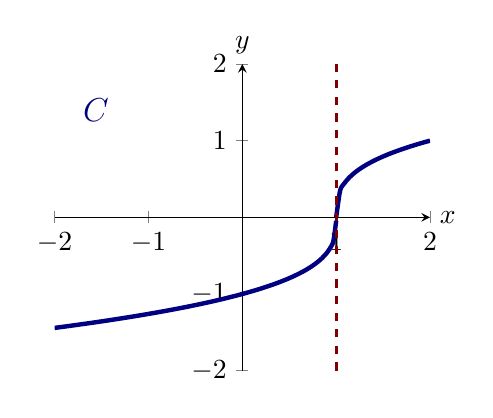
\begin{tikzpicture}
        \begin{axis}[
          domain=-2:2,
          xmin=-2, xmax=2,
          ymin=-2, ymax=2,
          width=2.5in,
          axis lines =middle, xlabel=$x$, ylabel=$y$,
          every axis y label/.style={at=(current axis.above origin),anchor=south},
          every axis x label/.style={at=(current axis.right of origin),anchor=west},
          ]
	  \addplot [ ultra thick, penColor, smooth,domain=(1:2)] {(x-1)^(1/3)};
	    \addplot [ultra thick, penColor, smooth,samples=100,domain=(-2:1)] {-(1-x)^(1/3)};
	
          \node at (axis cs:-1.8, 1.4 ) [penColor,anchor=west] {\large$C$};
  
              \addplot [very thick,penColor2,dashed] plot coordinates {(1,-2) (1,2)};
        \end{axis}
      \end{tikzpicture}
      &
      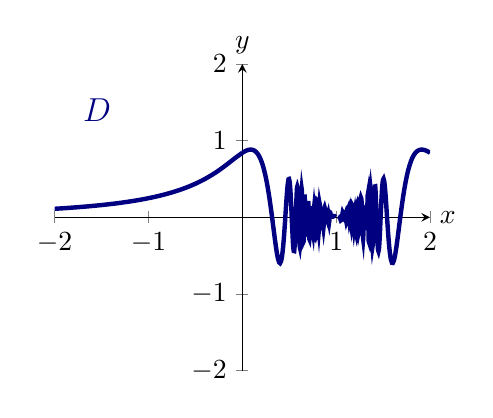
\begin{tikzpicture}
        \begin{axis}[
          domain=-2:2,
          xmin=-2, xmax=2,
          ymin=-2, ymax=2,
          width=2.5in,
          axis lines =middle, xlabel=$x$, ylabel=$y$,
          every axis y label/.style={at=(current axis.above origin),anchor=south},
          every axis x label/.style={at=(current axis.right of origin),anchor=west},
          ]
	  \addplot [ultra thick, penColor, smooth,samples=100, domain=(0:0.995)] {{(1-x)*sin(deg(1/(1-x)^3))}};
	   \addplot [ultra thick, penColor, smooth, domain=(-2:0)] {{(1-x)*sin(deg(1/(1-x)^3))}};
	    \addplot [ultra thick, penColor, smooth,samples=100, domain=(1.02:2)] {{(x-1)*sin(deg(1/(x-1)^3))}};
	%  \addplot[color=penColor,fill=penColor,only marks,mark=*] coordinates{(1,0)}; 
          \node at (axis cs:-1.8, 1.4 ) [penColor,anchor=west] {\large$D$};
           % \node at (axis cs:0., 1.8 ) [penColor,anchor=west] {\large$y=f(x)$};
          
        \end{axis}
      \end{tikzpicture}
    \end{tabular}
  \end{image}
 The function in figure A is not continuous at $a$, and, therefore, it is not differentiable there.

In figures $B$--$D$ the functions are continuous at $a$, but  in each case the limit
\[
 \lim_{x\to a} \frac{f(x)-f(a)}{x-a}
\]
does not exist, for a different reason.

In figure $B$
\[
 \lim_{x\to a^{+}} \frac{f(x)-f(a)}{x-a}\ne \lim_{x\to a^{-}} \frac{f(x)-f(a)}{x-a}.
\]

 
In figure $C$
\[
 \lim_{x\to a} \frac{f(x)-f(a)}{x-a}=\infty.
\]
In figure $D$
the two one-sided limits don't exist and neither one of them is infinity.

So, if  at the point $a$ a function either has a "jump" in the graph, or a corner, or what looks like a ``vertical tangent line", or if it rapidly oscillates near $a$, then the function is not differentiable at $a$.
\end{explanation}
\end{question}
\end{document}
